\documentclass[a4paper,oneside,12pt]{report}
\usepackage{fontspec}
\usepackage{setspace}
\usepackage{amsmath}
\usepackage{titling}
\usepackage{geometry}
\usepackage{listings}
\usepackage{xcolor}
\usepackage{float}
\usepackage{hyperref}
\usepackage{indentfirst}
\usepackage{url}
\usepackage{fancyhdr}
\usepackage{tocloft}
\usepackage{bookmark}
\usepackage{booktabs}
\usepackage{caption}
\usepackage{tikz}
\usetikzlibrary{positioning,shapes.geometric,arrows.meta,decorations.pathreplacing}

\setmainfont{texgyretermes-regular.otf}[
    BoldFont=texgyretermes-bold.otf,
    ItalicFont=texgyretermes-italic.otf,
    BoldItalicFont=texgyretermes-bolditalic.otf
]
\onehalfspacing
\geometry{left=3cm, right=2.5cm, top=2cm, bottom=2.5cm}
\sloppy

\definecolor{codegreen}{rgb}{0,0.6,0}
\definecolor{codegray}{rgb}{0.5,0.5,0.5}
\definecolor{codepurple}{rgb}{0.58,0,0.82}
\definecolor{backcolour}{rgb}{0.95,0.95,0.92}
\definecolor{darkblue}{rgb}{0,0,0.6}

\lstdefinestyle{commonstyle}{
    backgroundcolor=\color{backcolour},
    breakatwhitespace=false,
    breaklines=true,
    captionpos=b,
    keepspaces=true,
    numbers=left,
    numbersep=5pt,
    showspaces=false,
    showstringspaces=false,
    showtabs=false,
    tabsize=2,
    frame=single,
    basicstyle=\ttfamily\footnotesize,
    numberstyle=\tiny\color{codegray},
    columns=flexible,
    postbreak=\mbox{\textcolor{red}{$\hookrightarrow$}\space},
    breakindent=0pt,
    breakautoindent=false
}
\lstdefinestyle{bashstyle}{
    style=commonstyle,
    language=bash,
    commentstyle=\color{codegreen},
    keywordstyle=\color{darkblue},
    stringstyle=\color{codepurple}
}
\lstdefinestyle{yamlstyle}{
    style=commonstyle,
    commentstyle=\color{codegreen},
    keywordstyle=\color{darkblue},
    stringstyle=\color{codepurple}
}
\lstdefinestyle{dockerstyle}{
    style=commonstyle,
    commentstyle=\color{codegreen},
    keywordstyle=\color{darkblue},
    stringstyle=\color{codepurple}
}

\newcommand{\customfbox}[1]{%
  \setlength{\fboxsep}{0pt}%
  \setlength{\fboxrule}{0.5pt}%
  \fcolorbox{black}{white}{#1}%
}
\renewcommand{\figurename}{Gambar}
\renewcommand{\thefigure}{\arabic{figure}}
\hypersetup{
    colorlinks=true,
    linkcolor=black,
    filecolor=black,
    urlcolor=black,
    citecolor=black,
    pdftitle={Laporan KEPL Pertemuan 5},
    pdfpagemode=FullScreen,
    breaklinks=true
}
\pagestyle{fancy}
\fancyhf{}
\fancyfoot[C]{\thepage}
\renewcommand{\headrulewidth}{0pt}
\fancypagestyle{plain}{
    \fancyhf{}
    \fancyfoot[C]{\thepage}
    \renewcommand{\headrulewidth}{0pt}
}
\renewcommand{\contentsname}{Daftar Isi}
\renewcommand{\bibname}{Daftar Pustaka}
\renewcommand{\thechapter}{}
\renewcommand{\chaptername}{}
\renewcommand{\thesection}{\arabic{chapter}.\arabic{section}}
\renewcommand{\thesubsection}{\thesection.\arabic{subsection}}
\setcounter{secnumdepth}{3}
\setcounter{tocdepth}{3}
\renewcommand{\cftchapdotsep}{\cftdotsep}
\renewcommand{\cftchapleader}{\cftdotfill{\cftchapdotsep}}
\setlength{\cftchapindent}{0em}
\setlength{\cftsecindent}{2em}
\setlength{\cftsubsecindent}{4em}
\setlength{\cftchapnumwidth}{0em}
\setlength{\cftsecnumwidth}{2.5em}
\setlength{\cftsubsecnumwidth}{3.2em}
\renewcommand{\cftchappresnum}{}
\renewcommand{\cftchapaftersnum}{}
\newcommand{\tocboldsection}[1]{%
  \protect\renewcommand{\protect\cftchapfont}{\protect\bfseries}%
  #1%
  \protect\renewcommand{\protect\cftchapfont}{}%
}

\begin{document}

\newgeometry{left=3cm, right=2.5cm, top=2.5cm, bottom=3cm}
\begin{titlingpage}
\begin{spacing}{1}
\begin{center}
\vspace*{0.2cm}
{\large \textbf{\MakeUppercase{Laporan Praktikum}}} \\[0.4cm]
{\large \textbf{\MakeUppercase{Konstruksi dan Evolusi Perangkat Lunak}}} \\[0.4cm]
{\large \textbf{\MakeUppercase{Pertemuan 5}}} \\[0.4cm]
{\large \textbf{\MakeUppercase{Multi-Stage Docker Build dan Distribusi Image GHCR}}} \\[1.5cm]


\includegraphics[height=7cm]{images/UGM.png} \\[0.7cm]

{\normalsize \textbf{Disusun oleh:}} \\[0.4cm]
\begin{tabular}{@{}l l @{}}
  \textbf{Nama}           & : Hafidz Rizqullah Prasetya \\
  \textbf{NIM}            & : 24/535493/SV/24243 \\
  \textbf{Kelas}          & : PL5A1 \\
  \textbf{Dosen Pengampu} & : Galih Malela Damaraji \\
\end{tabular} \\[1.2cm]

{\normalsize \textbf{PROGRAM STUDI D-IV}} \\[0.2cm]
{\normalsize \textbf{TEKNOLOGI REKAYASA PERANGKAT LUNAK}} \\[0.2cm]
{\normalsize \textbf{DEPARTEMEN TEKNIK ELEKTRO DAN INFORMATIKA}} \\[0.2cm]
{\normalsize \textbf{SEKOLAH VOKASI}} \\[0.2cm]
{\normalsize \textbf{UNIVERSITAS GADJAH MADA}} \\[0.2cm]
{\normalsize \textbf{YOGYAKARTA}} \\[0.2cm]
{\normalsize \textbf{2026}} \\[1.2cm]
\end{center}
\end{spacing}
\end{titlingpage}
\restoregeometry

\thispagestyle{empty}
\clearpage
\stepcounter{page}
\thispagestyle{empty}

\addcontentsline{toc}{chapter}{Daftar Isi}
\tableofcontents
\clearpage

\pagenumbering{arabic}
\setcounter{page}{3}

\chapter[Tujuan Praktikum]{Tujuan Praktikum}
Sesuai arahan pada pertemuan kelima dan deskripsi tugas di Google Classroom mata kuliah \textit{Konstruksi dan Evolusi Perangkat Lunak 2026}, tujuan praktikum ini adalah:
\begin{enumerate}
    \item Mahasiswa mampu mengonversi berkas Dockerfile aplikasi Laravel dari model \textit{single-stage} menjadi \textit{multi-stage} build, memisahkan tahap instalasi dependensi dengan tahap eksekusi produksi.
    \item Mahasiswa mampu membuktikan penurunan ukuran container image secara terukur melalui perbandingan perintah \texttt{docker images} sebelum dan sesudah optimasi, lengkap dengan kalkulasi selisih megabyte serta persentasenya.
    \item Mahasiswa mampu mengunci versi \textit{base image} secara spesifik dan beralih ke varian ringan berbasis Alpine Linux guna meminimalkan jejak memori dan celah keamanan.
    \item Mahasiswa mampu mengonfigurasi instruksi \texttt{USER} non-root dan \texttt{HEALTHCHECK} pada container, serta membuktikannya melalui \texttt{docker exec} dan atribut \texttt{(healthy)} pada \texttt{docker ps}.
    \item Mahasiswa mampu menyusun workflow GitHub Actions untuk proses otomatisasi \textit{build} dan \textit{push} container image ke GitHub Container Registry (GHCR) dengan penandaan tag commit SHA dan visibilitas publik.
\end{enumerate}

\clearpage

\chapter{Dasar Teori}

\section{Konsep Multi-Stage Build pada Docker}
Pada tahap awal pembuatan image Docker, pendekatan konvensional \textit{single-stage} sering kali menggabungkan seluruh perkakas pembangun (compiler, paket \textit{development header}, dan manajer paket seperti Composer) ke dalam satu image akhir \cite{docker-docs}. Pendekatan ini menghasilkan ukuran image yang besar karena berkas-berkas sementara dan pustaka kompilasi ikut terbawa ke lingkungan produksi.

\textit{Multi-stage build} memecahkan persoalan ini dengan membagi instruksi Dockerfile ke dalam beberapa blok \texttt{FROM} yang berdiri sendiri \cite{docker-multistage}. Tahap pertama bertindak sebagai \textit{builder} yang bertugas mengunduh dependensi dan menyusun aset. Tahap kedua bertindak sebagai \textit{runtime} yang hanya menyalin hasil akhir (direktori \texttt{vendor} dan berkas aplikasi) dari tahap pertama tanpa menyertakan perkakas pembangun.

\begin{figure}[H]
    \centering
    \begin{tikzpicture}[
        font=\footnotesize,
        kotak/.style={draw, rounded corners=2pt, align=center, minimum height=1.1cm, minimum width=3.4cm, inner sep=4pt, fill=white},
        panah/.style={-{Latex[length=2.5mm]}, thick, draw=black!70},
        label/.style={font=\scriptsize, text=black!70},
    ]
    \node[kotak, fill=blue!10] (builder) at (0,0) {\textbf{Tahap 1: Builder}\\\texttt{composer:2.8.5}\\Composer, dev packages, cache};
    \node[kotak, fill=green!12] (runtime) at (6.5,0) {\textbf{Tahap 2: Runtime}\\\texttt{php:8.4.26-cli-alpine}\\Aplikasi bersih, runtime Alpine};
    \node[kotak, fill=orange!12] (image) at (12,0) {\textbf{Hasil Akhir}\\\texttt{ghcr.io/...:sha}\\Ukuran pangkas 71.7\%};

    \draw[panah] (builder) -- node[above, font=\scriptsize] {\texttt{COPY --from=builder}} node[below, font=\scriptsize] {hanya direktori \texttt{/app}} (runtime);
    \draw[panah] (runtime) -- node[above, font=\scriptsize] {build \& tag} (image);
    \end{tikzpicture}
    \caption{Alur pemisahan tahap builder dan tahap runtime pada multi-stage Docker build.}
    \label{fig:multistage}
\end{figure}

\section{Prinsip Least Privilege dan Keamanan Container}
Secara bawaan, proses di dalam container berjalan dengan hak akses \textit{root} (UID 0) jika instruksi \texttt{USER} tidak didefinisikan secara eksplisit. Menjalankan aplikasi web sebagai pengguna \textit{root} melanggar prinsip \textit{least privilege} dan memperbesar risiko keamanan apabila terjadi eksploitasi \textit{remote code execution} atau \textit{container breakout} ke mesin host \cite{docker-security}.

Penggunaan direktif \texttt{USER} menginstruksikan daemon Docker untuk menurunkan hak akses proses ke akun pengguna non-root (seperti \texttt{www-data}). Untuk aplikasi Laravel yang membutuhkan operasi tulis pada direktori penyimpanan lokal (seperti \texttt{storage}, \texttt{bootstrap/cache}, dan berkas SQLite), kepemilikan dan izin akses direktori harus disesuaikan terlebih dahulu sebelum hak akses proses dialihkan ke pengguna non-root.

\section{Mekanisme Pemeriksaan Kesehatan Container (Healthcheck)}
Instruksi \texttt{HEALTHCHECK} pada Dockerfile memberitahu Docker bagaimana cara memverifikasi bahwa aplikasi di dalam container tidak hanya sekadar berjalan sebagai proses, melainkan benar-benar mampu melayani permintaan jaringan secara normal \cite{docker-healthcheck}. 

Docker menjalankan perintah healthcheck secara periodik sesuai interval waktu yang ditentukan. Jika perintah menghasilkan kode keluar 0, container ditandai berstatus \texttt{healthy}. Sebaliknya, jika perintah mengembalikan nilai non-nol berulang kali hingga batas toleransi (\textit{retries}), container akan ditandai berstatus \texttt{unhealthy}. Informasi status ini krusial bagi sistem orkestrasi dan pengguna untuk mendeteksi kegagalan layanan secara dini.

\section{GitHub Container Registry (GHCR)}
GitHub Container Registry adalah layanan registri artefak OCI (Open Container Initiative) yang terintegrasi langsung dengan GitHub Packages \cite{github-ghcr}. GHCR memungkinkan pengembang mendistribusikan container image dengan kontrol akses berbasis repositori atau organisasi.

Melalui GitHub Actions, proses publikasi ke GHCR dapat diotomatisasi secara aman tanpa memerlukan token statis pihak ketiga. Workflow memanfaatkan variabel bawaan \texttt{secrets.GITHUB\_TOKEN} dengan cakupan izin \texttt{packages: write}. Penandaan image menggunakan tag commit hash (\texttt{\$\{\{ github.sha \}\}}) menjamin ketertelusuran (\textit{traceability}) antara berkas rilis image dengan riwayat kode sumber di repositori git.

\clearpage

\chapter{Alat dan Bahan}
Alat dan bahan yang digunakan pada praktikum pertemuan kelima ini adalah:
\begin{itemize}
    \item Perangkat komputer jinjing dengan sistem operasi Linux Ubuntu/Fedora kernel 6.14.
    \item Docker Engine versi 27 dan Docker Buildx.
    \item Git CLI dan GitHub CLI (\texttt{gh}) versi 2.65.
    \item Akun GitHub aktif atas nama \texttt{hafidzrizqullahprasetya}.
    \item Repositori proyek \texttt{evolusi-pl-535493} yang berisi aplikasi Laravel berbasis SQLite.
    \item Peramban web untuk verifikasi antarmuka GitHub Actions dan GitHub Container Registry.
\end{itemize}

\clearpage

\chapter{Langkah Kerja dan Implementasi}

\section{Analisis Baseline Image (Single-Stage)}
Sebelum melakukan perombakan berkas Dockerfile, saya menyiapkan satu berkas baseline \textit{single-stage} untuk mengukur kondisi awal ukuran image aplikasi Laravel. Pada model single-stage, base image yang digunakan adalah \texttt{php:8.4-cli} berbasis Debian. Berkas tersebut menginstal paket perkakas \texttt{git}, \texttt{unzip}, pustaka kompilasi ekstensi, serta mengunduh installer Composer utuh ke dalam image yang sama:

\begin{lstlisting}[style=dockerstyle,caption={Berkas baseline Dockerfile single-stage yang digunakan untuk pembanding.}]
FROM php:8.4-cli

WORKDIR /app

RUN apt-get update && apt-get install -y --no-install-recommends \
    git unzip libzip-dev libsqlite3-dev curl \
    && docker-php-ext-install pdo_sqlite zip bcmath \
    && rm -rf /var/lib/apt/lists/* \
    && curl -sS https://getcomposer.org/installer | php -- --install-dir=/usr/local/bin --filename=composer

COPY composer.json composer.lock ./
RUN composer install --no-dev --prefer-dist --no-interaction --no-scripts

COPY . .

RUN cp .env.example .env && \
    touch database/database.sqlite && \
    php artisan key:generate && \
    php artisan migrate --force

EXPOSE 8000
CMD ["php", "artisan", "serve", "--host=0.0.0.0", "--port=8000"]
\end{lstlisting}

Image baseline tersebut dibangun dengan tag \texttt{evolusi-pl-535493:single-stage}. Hasil pembacaan ukuran disk mencapai \textbf{940 MB}, yang mana ukuran tersebut tergolong sangat besar untuk sebuah layanan microservice aplikasi web.

\section{Pembuatan Berkas .dockerignore}
Untuk mencegah masuknya berkas-berkas yang tidak diperlukan ke dalam konteks build Docker, saya membuat berkas \texttt{.dockerignore} pada akar repositori. Berkas ini secara spesifik mengecualikan direktori lokal seperti \texttt{vendor}, \texttt{node\_modules}, riwayat git, dan berkas konfigurasi sementara:

\begin{lstlisting}[style=bashstyle,caption={Berkas \texttt{.dockerignore} pada repositori \texttt{evolusi-pl-535493}.}]
.git
.gitignore
.env
vendor
node_modules
frontend/node_modules
frontend/dist
storage/logs/*
!storage/logs/.gitignore
bootstrap/cache/*.php
tests
\end{lstlisting}

\section{Perancangan Multi-Stage Dockerfile}
Saya merombak berkas \texttt{Dockerfile} utama menjadi dua tahap terpisah:
\begin{enumerate}
    \item \textbf{Tahap Builder}: Menggunakan base image \texttt{composer:2.8.5}. Pada tahap ini, berkas \texttt{composer.json} dan \texttt{composer.lock} disalin terlebih dahulu guna memanfaatkan layer cache Docker. Perintah \texttt{composer install} dijalankan dengan opsi \texttt{--no-dev} dan \texttt{--optimize-autoloader}. Selanjutnya seluruh berkas aplikasi disalin dan dilakukan dump autoloader produksi.
    \item \textbf{Tahap Runtime}: Menggunakan base image minimal yang dikunci versinya, yaitu \texttt{php:8.4.26-cli-alpine}. Pustaka runtime yang disematkan hanya ekstensi \texttt{bcmath}. Berkas hasil build dari tahap pertama disalin menggunakan direktif \texttt{COPY --from=builder /app /app}.
\end{enumerate}

Selain pemisahan tahap, saya menambahkan konfigurasi hak akses non-root dan penanganan kesehatan container:
\begin{itemize}
    \item Perintah \texttt{chown -R www-data:www-data /app} dan penyesuaian izin direktori penyimpanan (\texttt{storage}, \texttt{bootstrap/cache}, dan \texttt{database}).
    \item Direktif \texttt{USER www-data} agar proses container tidak dijalankan sebagai akun root.
    \item Direktif \texttt{HEALTHCHECK} dengan interval 10 detik yang memanggil endpoint \texttt{/api/tugas} melalui utilitas \texttt{curl}.
\end{itemize}

Berikut adalah isi lengkap berkas \texttt{Dockerfile} multi-stage:

\begin{lstlisting}[style=dockerstyle,caption={Berkas Dockerfile multi-stage dengan versi Alpine terkunci dan non-root user.}]
# Tahap build: siapkan dependensi vendor tanpa paket dev
FROM composer:2.8.5 AS builder

WORKDIR /app

COPY composer.json composer.lock ./

RUN composer install \
    --no-dev \
    --prefer-dist \
    --no-interaction \
    --no-scripts \
    --optimize-autoloader

COPY . .

RUN composer dump-autoload --optimize --no-dev

# Tahap runtime: image minimal alpine dengan locked version dan non-root user
FROM php:8.4.26-cli-alpine

WORKDIR /app

RUN docker-php-ext-install -j$(nproc) bcmath

COPY --from=builder /app /app

RUN cp .env.example .env && \
    mkdir -p database storage/framework/sessions storage/framework/views storage/framework/cache storage/logs bootstrap/cache && \
    touch database/database.sqlite && \
    php artisan key:generate && \
    php artisan migrate --force && \
    chown -R www-data:www-data /app && \
    chmod -R 775 /app/storage /app/bootstrap/cache /app/database

USER www-data

EXPOSE 8000

HEALTHCHECK --interval=10s --timeout=3s --start-period=5s --retries=3 \
    CMD curl -f http://127.0.0.1:8000/api/tugas || exit 1

CMD ["php", "artisan", "serve", "--host=0.0.0.0", "--port=8000"]
\end{lstlisting}

\section{Pembuatan Workflow GitHub Actions ke GHCR}
Untuk mempublikasikan container image secara otomatis ke GitHub Container Registry saat kode digabungkan ke cabang utama, saya membuat berkas workflow baru pada direktori \texttt{.github/workflows/docker.yml}.

Workflow ini berjalan di lingkungan \texttt{ubuntu-latest} dengan izin \texttt{packages: write}. Nama image secara otomatis dikonversi ke huruf kecil agar memenuhi standar registri OCI, kemudian diautentikasi ke \texttt{ghcr.io} menggunakan token bawaan GitHub Actions. Tag image disematkan dalam dua format: nomor commit hash (\texttt{\$\{\{ github.sha \}\}}) dan tag \texttt{latest}.

\begin{lstlisting}[style=yamlstyle,caption={Berkas workflow GitHub Actions \texttt{.github/workflows/docker.yml}.}]
name: Docker

on:
  push:
    branches: [main, dev]
  workflow_dispatch:

permissions:
  contents: read
  packages: write

jobs:
  build-and-push:
    name: Build & Push GHCR
    runs-on: ubuntu-latest
    steps:
      - name: Checkout repository
        uses: actions/checkout@v4

      - name: Siapkan nama image huruf kecil
        run: echo "IMAGE_NAME=$(echo '${{ github.repository }}' | tr '[:upper:]' '[:lower:]')" >> $GITHUB_ENV

      - name: Login ke GitHub Container Registry
        run: echo "${{ secrets.GITHUB_TOKEN }}" | docker login ghcr.io -u "${{ github.actor }}" --password-stdin

      - name: Build Docker image
        run: |
          docker build \
            -t "ghcr.io/${IMAGE_NAME}:${{ github.sha }}" \
            -t "ghcr.io/${IMAGE_NAME}:latest" .

      - name: Push Docker image ke GHCR
        run: |
          docker push "ghcr.io/${IMAGE_NAME}:${{ github.sha }}"
          docker push "ghcr.io/${IMAGE_NAME}:latest"
\end{lstlisting}

\section{Pengelolaan Git dan Pull Request}
Karena cabang \texttt{main} pada repositori \texttt{evolusi-pl-535493} memiliki aturan proteksi cabang yang mewajibkan status check CI lulus sebelum penggabungan, alur kerja git dilakukan melalui mekanisme cabang fitur:
\begin{enumerate}
    \item Membuat cabang baru \texttt{feature/docker-multistage}.
    \item Melakukan commit berkas \texttt{.dockerignore}, \texttt{Dockerfile}, dan \texttt{.github/workflows/docker.yml} dengan pesan commit yang natural dan deskriptif.
    \item Mendorong cabang ke remote GitHub dan membuka Pull Request nomor 16 ke cabang \texttt{main}.
    \item Menunggu pemeriksaan workflow \texttt{CI} (job Build dan Test) selesai secara sukses.
    \item Melakukan merge Pull Request nomor 16 ke cabang \texttt{main}. Penggabungan ini langsung memicu eksekusi workflow \texttt{Docker} untuk mem-publish image ke GHCR.
\end{enumerate}

\clearpage

\chapter{Hasil dan Pembahasan}

\section{Perbandingan Ukuran Image Sebelum dan Sesudah}
Pengujian pertama dilakukan dengan membandingkan ukuran fisik image yang terdaftar di daemon Docker lokal. Hasil perintah \texttt{docker images} menunjukkan perbedaan ukuran yang sangat signifikan antara image single-stage dan image multi-stage:

\begin{figure}[H]
    \centering
    \customfbox{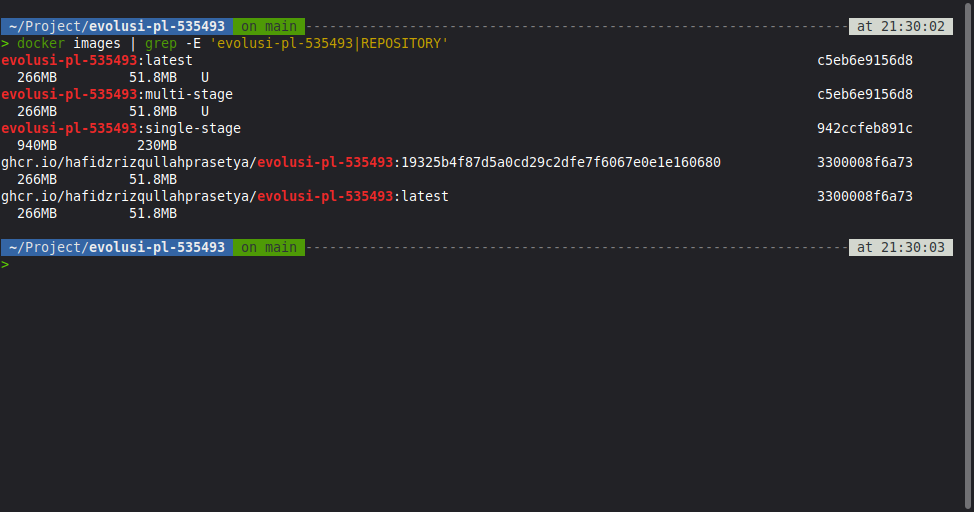
\includegraphics[width=0.98\textwidth]{images/ss-01-docker-images.png}}
    \caption{Perbandingan ukuran container image antara single-stage (940 MB) dan multi-stage (266 MB).}
    \label{fig:docker-images}
\end{figure}

Tabel berikut merangkum data perbandingan ukuran image sebelum dan sesudah optimasi:

\begin{table}[H]
\centering
\caption{Kalkulasi penurunan ukuran container image aplikasi Laravel.}
\label{tab:ukuran}
\begin{tabular}{@{}llcc@{}}
\toprule
\textbf{Nama Image} & \textbf{Tag} & \textbf{Ukuran Disk} & \textbf{Ukuran Konten} \\
\midrule
\texttt{evolusi-pl-535493} & \texttt{single-stage} & 940 MB & 230 MB \\
\texttt{evolusi-pl-535493} & \texttt{multi-stage}  & 266 MB & 51.8 MB \\
\texttt{evolusi-pl-535493} & \texttt{latest}       & 266 MB & 51.8 MB \\
\bottomrule
\end{tabular}
\end{table}

Kalkulasi selisih dan persentase efisiensi ukuran:
\begin{itemize}
    \item \textbf{Selisih Penurunan Ukuran:}
    \[
    \Delta \text{Ukuran} = 940\,\text{MB} - 266\,\text{MB} = 674\,\text{MB}
    \]
    \item \textbf{Persentase Penurunan:}
    \[
    \text{Efisiensi} = \left( \frac{674\,\text{MB}}{940\,\text{MB}} \right) \times 100\% = 71{,}70\%
    \]
\end{itemize}

Penurunan ukuran sebesar \textbf{71,70\%} (menghemat 674 MB) tercapai karena lingkungan runtime Alpine Linux membuang seluruh perkakas kompilasi C, cache composer, serta paket-paket sistem Debian yang tidak diperlukan oleh aplikasi saat melayani request.

\section{Verifikasi Identitas Pengguna Non-Root}
Sesuai arahan instruksi praktikum, container tidak boleh dijalankan dengan hak akses root. Saya menjalankan container bernama \texttt{evolusi-pl-app} di latar belakang dan memeriksa identitas pengguna yang aktif melalui perintah \texttt{docker exec}:

\begin{figure}[H]
    \centering
    \customfbox{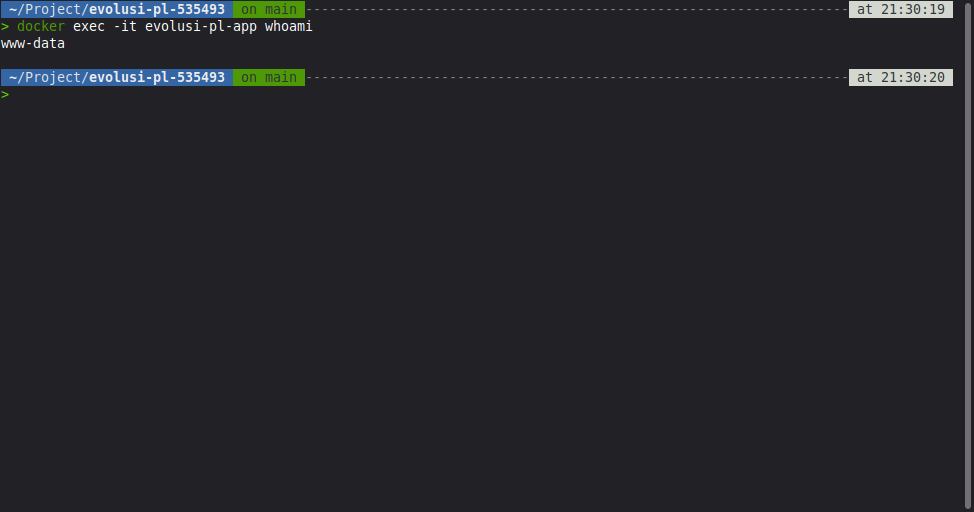
\includegraphics[width=0.98\textwidth]{images/ss-02-whoami.png}}
    \caption{Eksekusi perintah \texttt{docker exec -it evolusi-pl-app whoami} membuktikan proses berjalan sebagai user \texttt{www-data}.}
    \label{fig:whoami}
\end{figure}

Keluaran terminal secara tegas menampilkan \texttt{www-data}. Hal ini membuktikan bahwa instruksi \texttt{USER www-data} pada Dockerfile berhasil aktif dan proses aplikasi tidak memiliki hak akses administrator di dalam container.

\section{Verifikasi Status Kesehatan Container (Healthy)}
Pemeriksaan kesehatan container diuji menggunakan perintah \texttt{docker ps}. Setelah container berjalan melampaui masa \textit{start-period} (5 detik) dan interval pemeriksaan berkala pertama (10 detik), status container dipantau:

\begin{figure}[H]
    \centering
    \customfbox{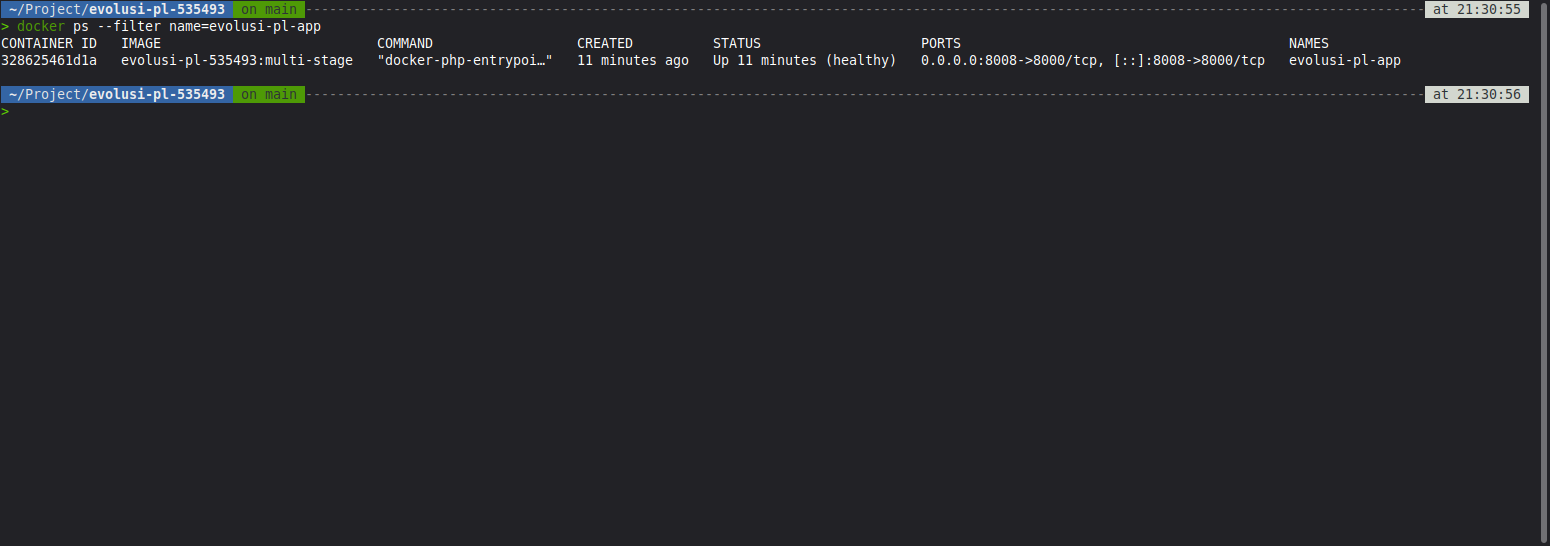
\includegraphics[width=0.98\textwidth]{images/ss-03-healthy.png}}
    \caption{Keluaran \texttt{docker ps} menampilkan status container \texttt{Up ... (healthy)}.}
    \label{fig:healthy}
\end{figure}

Pada Gambar \ref{fig:healthy}, kolom \texttt{STATUS} menampilkan penanda \texttt{(healthy)}. Ini membuktikan bahwa mekanisme pemanggilan endpoint \texttt{http://127.0.0.1:8000/api/tugas} via utilitas \texttt{curl} di dalam container berhasil dieksekusi secara periodik dan selalu mengembalikan kode respon sukses.

\section{Pengujian Endpoint API dari Luar Container}
Container dijalankan dengan memetakan port host 8008 ke port container 8000. Untuk menguji fungsionalitas aplikasi dari sisi klien luar, saya melakukan panggilan HTTP GET ke endpoint \texttt{/api/tugas} menggunakan utilitas \texttt{curl}:

\begin{figure}[H]
    \centering
    \customfbox{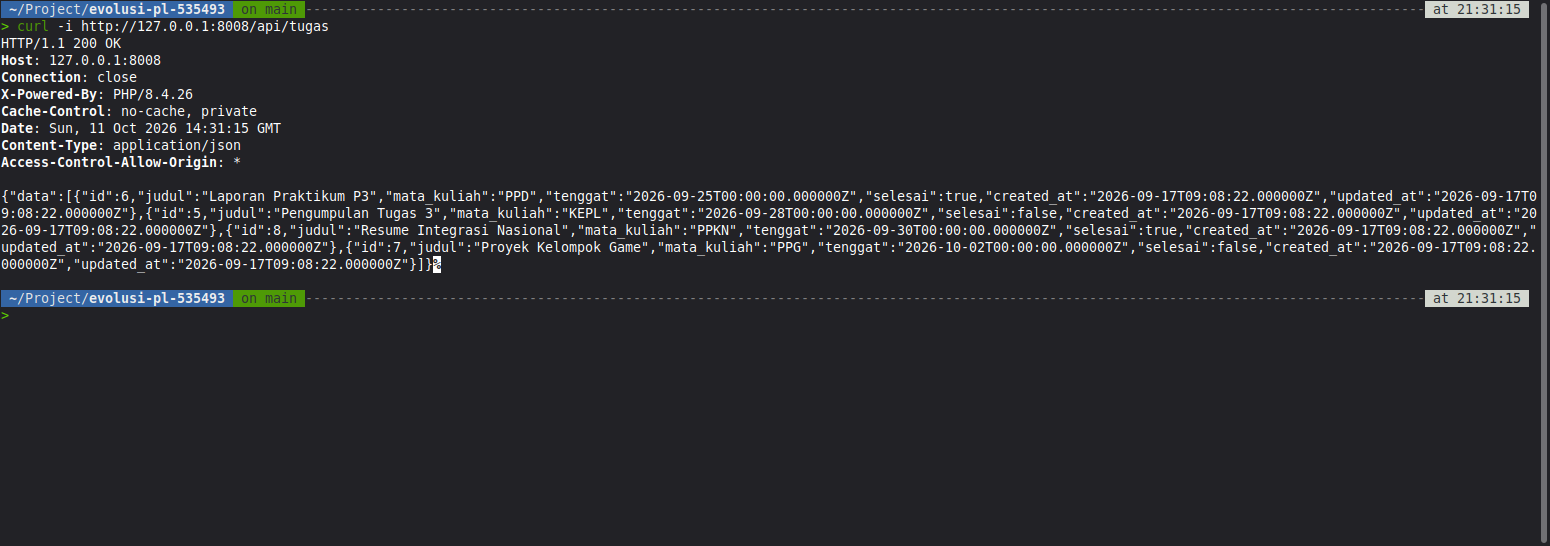
\includegraphics[width=0.98\textwidth]{images/ss-04-curl.png}}
    \caption{Pengujian pemanggilan API \texttt{/api/tugas} dari luar container menghasilkan status HTTP 200 OK beserta payload JSON.}
    \label{fig:curl}
\end{figure}

Respon yang diterima menunjukkan kode \texttt{HTTP/1.1 200 OK} dengan header \texttt{Content-Type: application/json}. Data JSON yang memuat daftar entitas tugas berhasil diambil dari basis data SQLite di dalam container tanpa hambatan izin baca-tulis.

\section{Bukti Eksekusi Workflow GitHub Actions}
Setelah Pull Request nomor 16 digabungkan ke cabang \texttt{main}, workflow \texttt{Docker} secara otomatis dijalankan oleh runner GitHub Actions. Gambar \ref{fig:actions} memperlihatkan log eksekusi workflow yang berhasil diselesaikan dengan status hijau:

\begin{figure}[H]
    \centering
    \customfbox{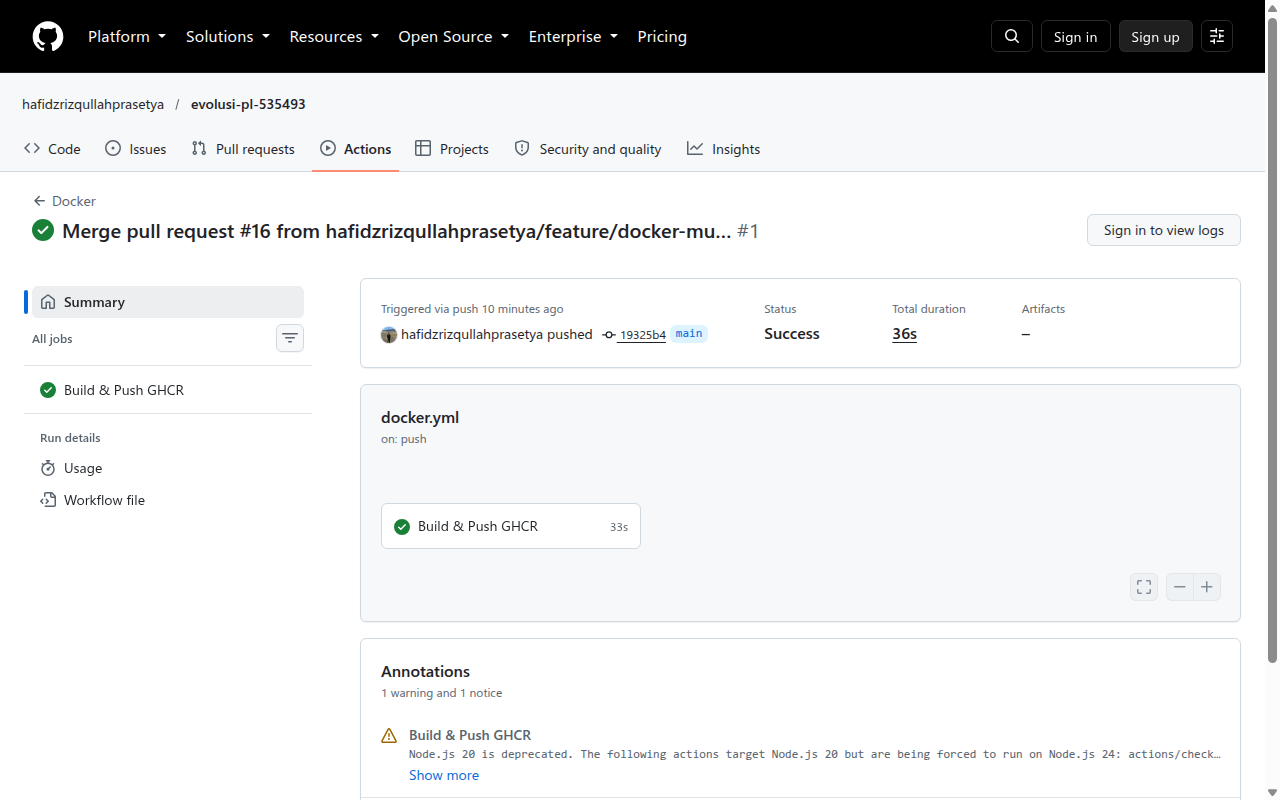
\includegraphics[width=0.98\textwidth]{images/ss-05-workflow-actions.png}}
    \caption{Tampilan antarmuka GitHub Actions membuktikan eksekusi workflow \texttt{Docker} berjalan sukses (hijau) dalam 33 detik.}
    \label{fig:actions}
\end{figure}

Job \texttt{Build \& Push GHCR} sukses menyelesaikan seluruh tahapan: mulai dari persiapan variabel repositori, autentikasi ke registri \texttt{ghcr.io}, build image multi-stage, hingga proses push dua tag image ke GitHub Container Registry.

\section{Bukti Publikasi Package di GitHub Container Registry}
Hasil akhir publikasi dapat dilihat langsung pada tab Packages di repositori GitHub \texttt{hafidzrizqullahprasetya/evolusi-pl-535493}:

\begin{figure}[H]
    \centering
    \customfbox{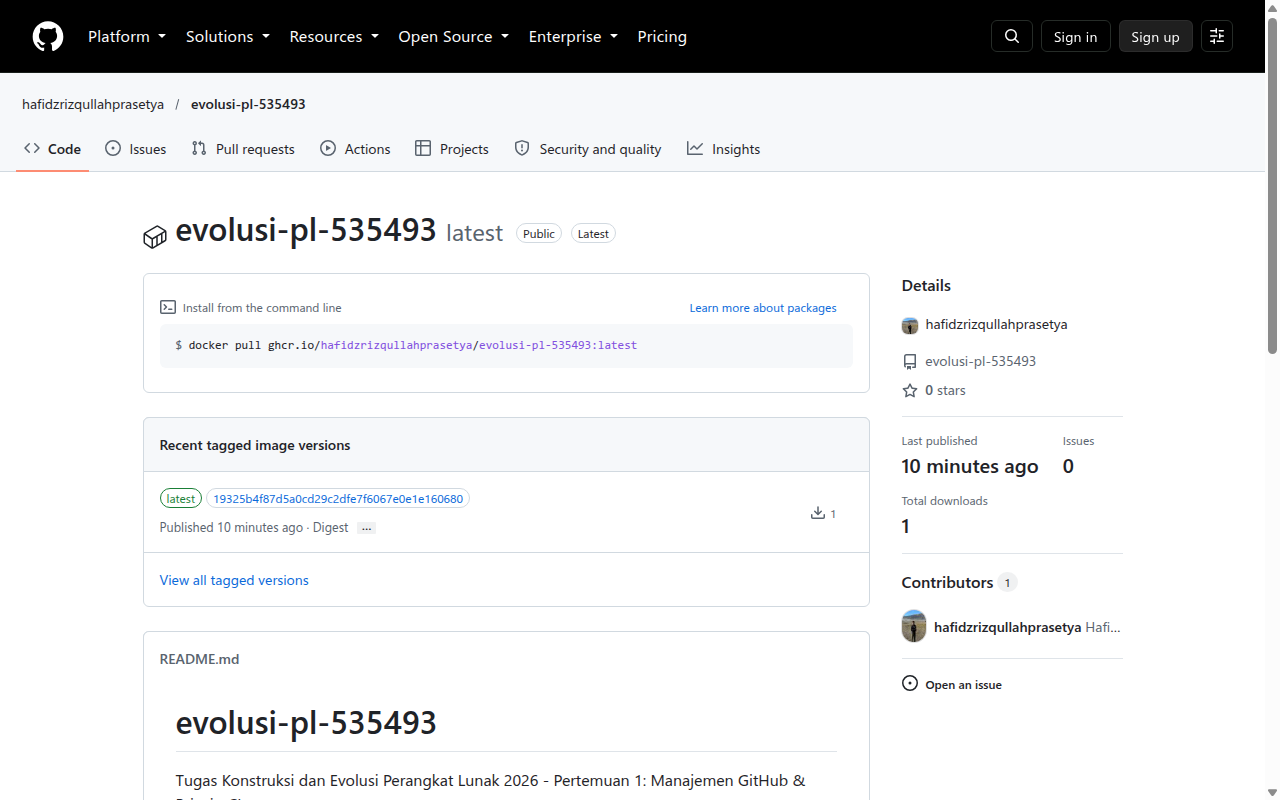
\includegraphics[width=0.98\textwidth]{images/ss-06-ghcr-package.png}}
    \caption{Halaman package \texttt{evolusi-pl-535493} di GitHub Container Registry dengan visibilitas Public.}
    \label{fig:package}
\end{figure}

Pada halaman tersebut terlihat rincian paket container:
\begin{itemize}
    \item Nama paket: \texttt{evolusi-pl-535493}.
    \item Status visibilitas: \textbf{Public} (dapat diunduh secara bebas oleh publik tanpa autentikasi).
    \item Tag rilis aktif: \texttt{latest} dan \texttt{19325b4f87d5a0cd29c2dfe7f6067e0e1e160680} (sesuai nomor commit push pada cabang main).
    \item Perintah instalasi publik:
    \begin{lstlisting}[style=bashstyle]
docker pull ghcr.io/hafidzrizqullahprasetya/evolusi-pl-535493:latest
    \end{lstlisting}
\end{itemize}

\clearpage

\chapter{Kesimpulan}
Berdasarkan serangkaian langkah praktikum dan pengujian yang telah dilaksanakan pada pertemuan kelima ini, diperoleh kesimpulan sebagai berikut:
\begin{enumerate}
    \item Penerapan arsitektur \textit{multi-stage build} berhasil memisahkan tahap persiapan dependensi Composer dari tahap runtime produksi, sehingga berkas sampah kompilasi tidak mengotori lingkungan rilis.
    \item Penggunaan base image minimal berbasis \texttt{php:8.4.26-cli-alpine} berhasil memangkas ukuran container image secara drastis dari \textbf{940 MB} menjadi \textbf{266 MB}, menghasilkan penurunan ukuran sebesar \textbf{674 MB} atau setara dengan efisiensi \textbf{71,70\%}.
    \item Aspek keamanan container meningkat dengan diterapkannya instruksi \texttt{USER www-data}, memastikan container tidak beroperasi dengan privilese akun \textit{root}.
    \item Mekanisme \texttt{HEALTHCHECK} berhasil mengawasi keandalan layanan web secara otomatis di dalam container, yang dibuktikan dengan status \texttt{(healthy)} pada pemantauan \texttt{docker ps}.
    \item Jalur CI/CD untuk pengiriman artefak container berhasil diotomatisasi melalui GitHub Actions, menghasilkan publikasi image ke GitHub Container Registry (GHCR) dengan tag penanda commit SHA serta visibilitas publik yang dapat diakses secara terbuka.
\end{enumerate}

\vspace{0.8cm}
\noindent\textbf{Tautan Pengumpulan Praktikum:}
\begin{itemize}
    \item Repositori Proyek: \url{https://github.com/hafidzrizqullahprasetya/evolusi-pl-535493}
    \item Halaman Package GHCR: \url{https://github.com/hafidzrizqullahprasetya/evolusi-pl-535493/pkgs/container/evolusi-pl-535493}
\end{itemize}

\clearpage

\addcontentsline{toc}{chapter}{Daftar Pustaka}
\begin{thebibliography}{99}
    \bibitem{docker-docs} Docker Inc., ``Docker overview.'' [Online]. Tersedia: \url{https://docs.docker.com/get-started/overview/}.
    \bibitem{docker-multistage} Docker Inc., ``Multi-stage builds.'' [Online]. Tersedia: \url{https://docs.docker.com/build/building/multi-stage/}.
    \bibitem{docker-security} Docker Inc., ``Docker security and best practices.'' [Online]. Tersedia: \url{https://docs.docker.com/engine/security/}.
    \bibitem{docker-healthcheck} Docker Inc., ``HEALTHCHECK directive reference.'' [Online]. Tersedia: \url{https://docs.docker.com/reference/dockerfile/#healthcheck}.
    \bibitem{github-ghcr} GitHub Docs, ``Working with the Container registry.'' [Online]. Tersedia: \url{https://docs.github.com/en/packages/working-with-a-github-packages-registry/working-with-the-container-registry}.
    \bibitem{laravel-deployment} Laravel LLC, ``Deployment - Laravel 12.x Documentation.'' [Online]. Tersedia: \url{https://laravel.com/docs/deployment}.
\end{thebibliography}

\end{document}
